\chapter{Design and Implementation}
\label{cha:implementation}
implement canvas fingerprinting -> intresting and has many different aspects


* hashes are used to reduce the amount of data for fast and easy comparison (among other uses).
* small variations and differences in the input that are not noticeable to the human eye
* hashing functions are non-reversible

(\textcite{multilogin17})

* canvas fingerprinting starts when rendering canvas
* all fonts contain glyphs ->  set of paths or closed curves that are specified using a particular mathematical formula. 
* e.g. lower case “i” has two glyphs, one for the dot and one for the body
* These particular glyphs, which are also known as outlines, are then filled with pixels to create the final letter form.
(\textcite{multilogin17})

What makes each canvas fingerprint unique is not the final image that we see, but how each computer renders hinting and anti-aliasing.
* hinting: Hints are basically instructions that are executed when the glyphs are drawn on your screen. These instructions move some of the points which define the shape of the letters, in order to make sure they are positioned correctly in relation to the grid where the glyph is displayed. This way, the font will look the same regardless of what screen it’s displayed on.
* anti-alisaing: may be the most common filter used today, and it consists of using gray pixels to smudge the edges of each glyph. If you zoom into a page, you’ll notice that the edges of curved letters are not perfect, but are rather jagged. The anti-aliasing filter smoothes out these jagged edges because our eyes average out the difference in tonality.
(\textcite{multilogin17})

* Note that scientific studies indicate that computer hardware, drivers, and browser versions can all affect the resulting glyphs. Also, in our own research, we’ve noticed that computers with the same graphic processing units (GPUs) will likely produce the same results.
(\textcite{multilogin17})

Canvas device fingerprinting has a sizable benefit over other traditional methods, in that it changes much slower than other prints. For example, if you are on Firefox 30 and upgrade to Firefox 42, the print will remain the same. This is due to the fact that the canvas element is essentially device pritning the rendering engine, the graphics driver and GPU. 
(\textcite{jkula17})

 draw text on the screen in a hidden box
(\textcite{jkula17})\\


\section{Idea}

\section{Architecture}

\subsection{Application scenario}

This chapter discusses the techniques introduced in \autoref{sec:Techniques} in form of a small application scenario. It concludes with a comparison which mounts to the one technique which is used for the prototype in \hyperref[cha:implementation]{chapter 5}.

\begin{figure}[H]
	\centering
	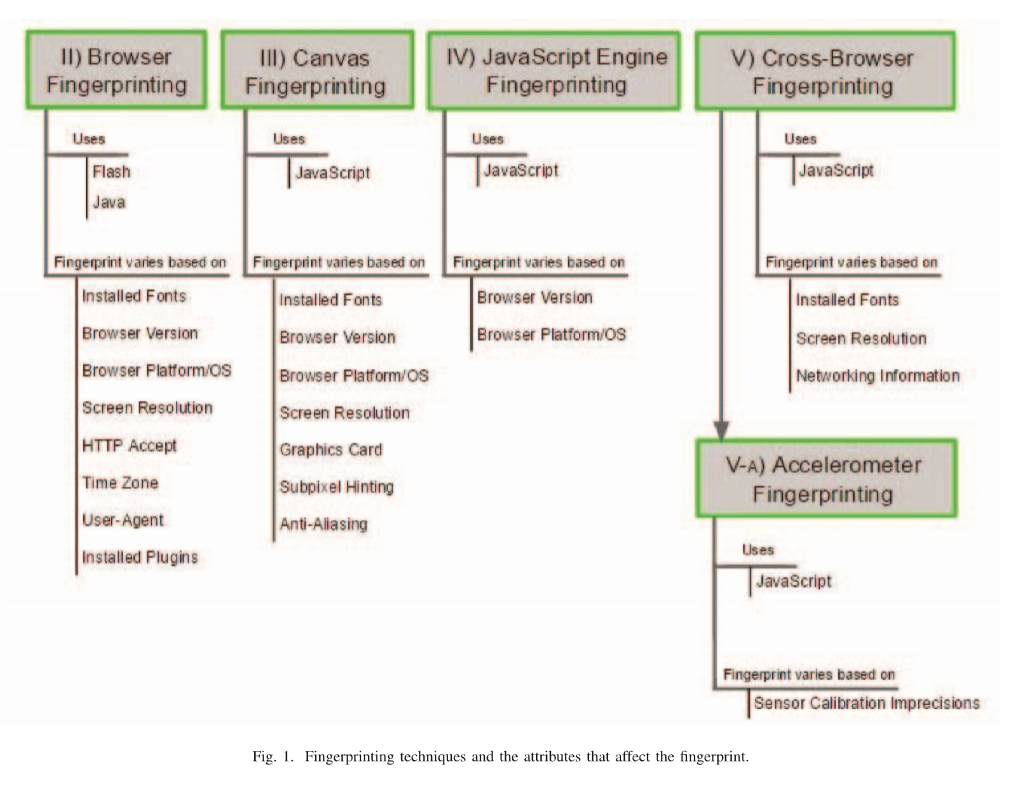
\includegraphics[width=350pt, height=160pt]{FingerprintingAttributes.png}
	\caption{Fingerprinting techniques and the attributes that effect the fingerprint}
	\label{BrowserSpecification}
\end{figure}

-- refere to previous chapter
-- give good overview what needs what?

In the figure below (1) the browser is requested to draw text on the screen in a hidden box. This text is enlarged, drawn in multiple colors and consists of a large range of text samples. Next (2) the drawing is converted to a base64 URL. Finally, (3) in order to shorten the output the base64 URL is hashed. This output is then used as the canvas device fingerprint. 
(\textcite{jkula17})\\

js.file -> FillText()/FillStyle()/FillRect()... -> Browser
js.file <- toDataURL() <- Browser
js.file -> Hash() to Database
(\textcite{jkula17})

\section{Programming}

the hash will be written into a json which is saved to a local file
the json will be updated whenever the user retries the fingerprint

* muss in chrome den zugriff auf lokale dateien extrig freigeben für die Speicherung der Daten
-- C:\Users\mayer.LAPTOP-T80OEI65\AppData\Local\Vivaldi\Application>vivaldi.exe --args --allow-file-access-from-file

* new idea: save data in google drive -> accessable from everywhere, at the same time
* further as javascript can not directly save/update files in the local file storage

* use servlet : https://www.youtube.com/watch?v=GO1Wi1nWuJM
* connect servlet with jsp with help of ajax: https://www.youtube.com/watch?v=P4eOHI6OGks

\section{Obtained Data}


\section{Fingerprint}

\subsection{Calculation}

\section{Visualisation}